\clearpage
\section{Solution Description}
\label{sec:solution}

\subsection{Design Assumptions}

The proposed pipeline constructs overlapping windows with a~fixed XY extent and the full local height. Here, \emph{voxel-based} describes external partitioning; RandLA-Net still receives individual points with XYZ coordinates and intensity. Sampling adjusts each input to the configured point count, $P$. The reference probability-sampling pipeline instead selects fixed-cardinality k-NN neighborhoods according to accumulated coverage, so their spatial extent varies with density. Both workflows combine repeated predictions and reconstruct labels for the original cloud.

\subsection{Pipeline Structure}

Figures~\ref{fig:voxel_pipeline} and~\ref{fig:probability_pipeline} show input construction, prediction aggregation, and full-cloud reconstruction for the two workflows.

\begin{figure}[H]
  \centering
  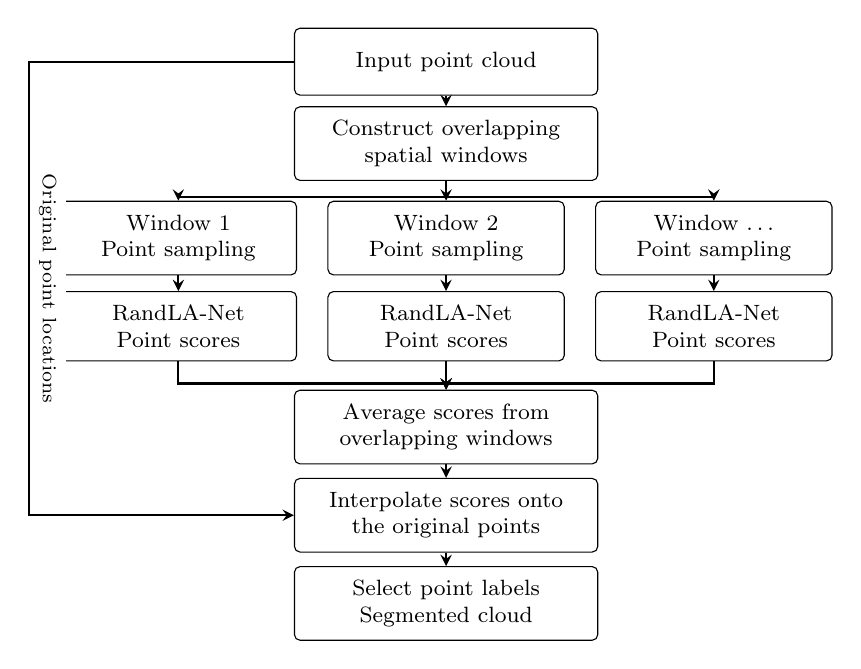
\begin{tikzpicture}[y=0.8cm,
    stage/.style={draw, rounded corners=2pt, align=center, text width=3.5cm,
      minimum height=0.85cm, inner sep=5pt, font=\footnotesize},
    branch/.style={stage, text width=2.65cm},
    flow/.style={->, thick, >=stealth}
  ]
    \node[stage] (input) at (0,0) {Input point cloud};
    \node[stage] (partition) at (0,-1.3) {Construct overlapping\\spatial windows};
    \node[branch] (window1) at (-3.4,-2.8) {Window 1\\Point sampling};
    \node[branch] (window2) at (0,-2.8) {Window 2\\Point sampling};
    \node[branch] (window3) at (3.4,-2.8) {Window $\ldots$\\Point sampling};
    \node[branch] (predict1) at (-3.4,-4.2) {RandLA-Net\\Point scores};
    \node[branch] (predict2) at (0,-4.2) {RandLA-Net\\Point scores};
    \node[branch] (predict3) at (3.4,-4.2) {RandLA-Net\\Point scores};
    \node[stage] (merge) at (0,-5.8) {Average scores from\\overlapping windows};
    \node[stage] (reconstruct) at (0,-7.2) {Interpolate scores onto\\the original points};
    \node[stage] (output) at (0,-8.6) {Select point labels\\Segmented cloud};

    \draw[flow] (input) -- (partition);
    \draw[flow] (partition.south) -- ++(0,-0.25) -| (window1.north);
    \draw[flow] (partition) -- (window2);
    \draw[flow] (partition.south) -- ++(0,-0.25) -| (window3.north);
    \draw[flow] (window1) -- (predict1);
    \draw[flow] (window2) -- (predict2);
    \draw[flow] (window3) -- (predict3);
    \draw[flow] (predict1.south) -- ++(0,-0.35) -| (merge.north);
    \draw[flow] (predict2) -- (merge);
    \draw[flow] (predict3.south) -- ++(0,-0.35) -| (merge.north);
    \draw[flow] (merge) -- (reconstruct);
    \draw[flow] (reconstruct) -- (output);
    \draw[flow] (input.west) -- (-5.3,0) -- (-5.3,-7.2)
      node[midway, above, sloped, font=\scriptsize, fill=white] {Original point locations}
      -- (reconstruct.west);
  \end{tikzpicture}
  \caption{Voxel-based pipeline. Overlapping windows provide separate model inputs, whose point scores are combined before reconstruction and label selection. The branches show repeated processing of spatial windows.\label{fig:voxel_pipeline}}
\end{figure}

The proposed pipeline first centers the cloud. Large clouds are processed in outer XY tiles without an overlap margin; smaller clouds are processed directly. Within each processing unit, a~regular grid generates windows with 40\% overlap along each horizontal axis. Windows containing more than $P$ points are reduced with bucket-based farthest point sampling (FPS). Those containing between $\lfloor P/4\rfloor$ and $P-1$ points are filled by random sampling with replacement. Windows with fewer points bypass the model and contribute zero score vectors.

Each model input is centered at its sampled-point mean and concatenated with intensity. The network returns class scores (logits), without a~final softmax. Repeated indices introduced by padding are reduced to one occurrence per window before accumulation. Scores for the same original point are then averaged across windows. A~KDTree over the retained points transfers these averaged scores to the processing unit's points using a~normalized Gaussian-weighted sum over up to 14 neighbors, with a~distance scale of 0.35~m. The class with the largest interpolated score is selected. Reconstruction uses CPU worker processes with shared coordinate and score arrays; each worker builds its own KDTree.

% \clearpage
\begin{figure}[H]
  \centering
  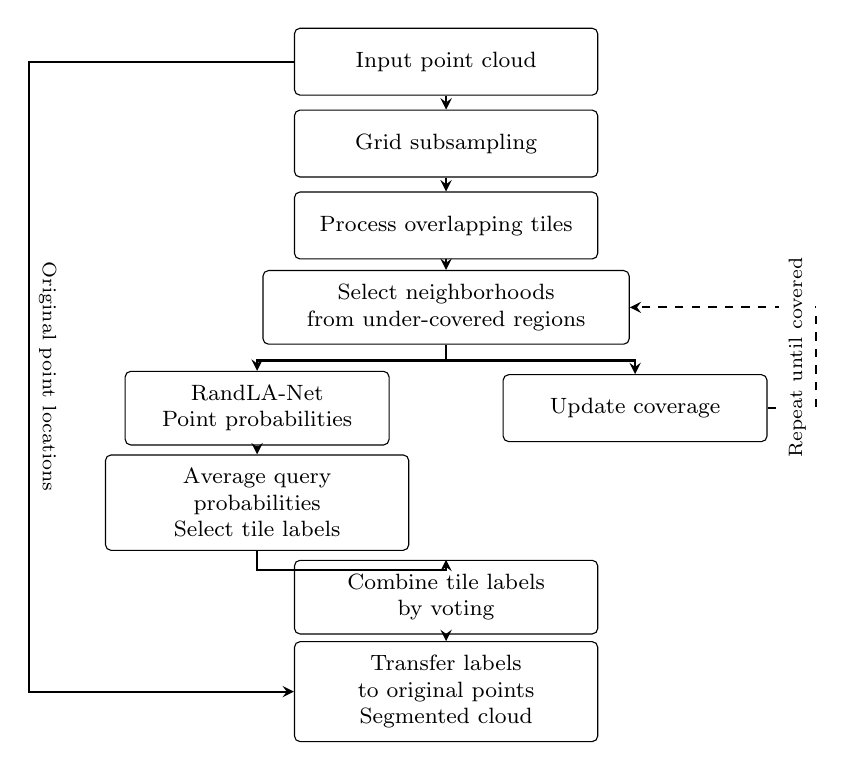
\begin{tikzpicture}[y=0.8cm,
    stage/.style={draw, rounded corners=2pt, align=center, text width=3.5cm,
      minimum height=0.85cm, inner sep=5pt, font=\footnotesize},
    flow/.style={->, thick, >=stealth}
  ]
    \node[stage] (input) at (0,0) {Input point cloud};
    \node[stage] (reduce) at (0,-1.3) {Grid subsampling};
    \node[stage] (tiles) at (0,-2.6) {Process overlapping tiles};
    \node[stage, text width=4.3cm] (query) at (0,-3.9) {Select neighborhoods\\from under-covered regions};
    \node[stage, text width=3cm] (predict) at (-2.4,-5.5) {RandLA-Net\\Point probabilities};
    \node[stage, text width=3cm] (coverage) at (2.4,-5.5) {Update coverage};
    \node[stage] (aggregate) at (-2.4,-7) {Average query probabilities\\Select tile labels};
    \node[stage] (vote) at (0,-8.5) {Combine tile labels\\by voting};
    \node[stage] (output) at (0,-10) {Transfer labels to original points\\Segmented cloud};

    \draw[flow] (input) -- (reduce);
    \draw[flow] (reduce) -- (tiles);
    \draw[flow] (tiles) -- (query);
    \draw[flow] (query.south) -- ++(0,-0.25) -| (predict.north);
    \draw[flow] (query.south) -- ++(0,-0.25) -| (coverage.north);
    \draw[flow, dashed] (coverage.east) -- (4.7,-5.5) -- (4.7,-3.9)
      node[midway, above, sloped, font=\scriptsize, fill=white] {Repeat until covered}
      -- (query.east);
    \draw[flow] (predict) -- (aggregate);
    \draw[flow] (aggregate.south) -- ++(0,-0.3) -| (vote.north);
    \draw[flow] (vote) -- (output);
    \draw[flow] (input.west) -- (-5.3,0) -- (-5.3,-10)
      node[midway, above, sloped, font=\scriptsize, fill=white] {Original point locations}
      -- (output.west);
  \end{tikzpicture}
  \caption{Probability-sampling pipeline. Neighborhood prediction and coverage tracking accompany repeated queries within each tile. Query probabilities are combined into tile labels, followed by voting across tiles and label transfer to the original cloud.\label{fig:probability_pipeline}}
\end{figure}

The probability-sampling pipeline instead begins with three-dimensional grid subsampling, retaining the measured point nearest each occupied cell center. The reduced cloud is divided into overlapping XY tiles. Within a~tile, query centers are selected in batches from the points with the lowest possibility values, and k-NN queries retrieve up to $P$ distinct neighbors per center. Smaller neighborhoods are padded by repetition for model input. Possibility increments decrease with distance from the center, and queries continue until the minimum possibility reaches the configured threshold. This threshold controls accumulated coverage weights rather than an exact number of observations. Softmax probabilities are averaged across queries before a~tile-level class decision; overlapping tiles are combined by hard voting. Finally, a~1-NN search transfers the resulting labels to the original cloud.

\subsection{Computational Complexity and Pipeline Limitations}

For a~processing unit with $N$ points and $W$ candidate windows, window selection requires $O(NW)$ point-in-window checks. Sampling and model inference add work for each populated window. Score accumulation and reconstruction require storage proportional to $NC$, where $C$ is the number of classes, in addition to coordinates and spatial indices. Outer tiling bounds the spatial extent handled at once, although the complete input cloud remains in memory.

The proposed workflow processes a~finite grid of windows, whereas the number of probability-sampling queries depends on how quickly the possibility threshold is reached. Increasing window overlap adds repeated observations and model calls. Window size controls the available spatial context, but does not remove dependence on density: dense windows are reduced, intermediate windows are padded, and very sparse windows bypass inference. Reconstruction also introduces a~choice between combining neighboring score vectors before classification and transferring a~single neighboring label. The effects of these choices on segmentation quality and resource consumption require experimental evaluation.
